\documentclass[conference]{IEEEtran}

\IEEEoverridecommandlockouts

\usepackage[utf8]{inputenc}
\usepackage[T1]{fontenc}

\usepackage{cite}

\ifCLASSINFOpdf
  \usepackage[pdftex]{graphicx}

\else

\fi

\usepackage[cmex10]{amsmath}

\usepackage{multirow}
\usepackage{array}
\usepackage[lofdepth,lotdepth]{subfig}
\usepackage{color}
\usepackage{tabto}

\usepackage{amssymb}
\usepackage{booktabs}
\usepackage{multirow}
\usepackage{rotating}
\usepackage{amsmath}
\usepackage{algorithm}
\usepackage{algpseudocode}
\usepackage{lineno,hyperref}
\usepackage{graphicx}
\usepackage{pdflscape}
\usepackage[none]{hyphenat}

\begin{document}

\IEEEpubid{\makebox[\columnwidth]{\hfill} \hspace{\columnsep}\makebox[\columnwidth]{}}

\title{Kırmızı Şarap Kalitesinin Makine Öğrenmesi Kullanılarak Tahmin Edilmesi
\\
\*

Predicting Red Wine Quality Using Machine Learning
}
\author{
	
\IEEEauthorblockN{Mehtap ÖKLÜ}
\IEEEauthorblockA{Bilgisayar Mühendisliği\\
	17110131052\\
	Kahramanmaraş Sütçü İmam Üniversitesi\\
	Kahramanmaraş, Türkiye\\
	mehtap\_oklu\_06@hotmail.com
	}
\and
\IEEEauthorblockN{Banu KÖSE}
\IEEEauthorblockA{Bilgisayar Mühendisliği\\
	18110131011\\
	Kahramanmaraş Sütçü İmam Üniversitesi\\
	Kahramanmaraş, Türkiye\\
	banukose1561@gmail.com
	}
}
\maketitle
\thispagestyle{plain}
\pagestyle{plain}
\begin{ozet}
Şarap, çok eski tarihlerden beri tüketilen, batı toplumlarında mutfakla özdeşleşmiş olan alkollü bir içecektir. Farklı meyvelerle üretilebiliyor olsa da, şarap denince akla ilk gelen meyve üzümdür. Şarap, çok geniş bir skalaya sahiptir. Bu yüzden her şarabın kalite oranı farklıdır. Üzümle üretilen şaraplardan biri de kırmızı şaraptır. Kırmızı şaraba ait bazı özniteliklerin (alkol oranı, pH, klorür vb.) değerleri incelenerek şarabın kalitesi tahmin edilebilir. Bu değerlerin incelenmesi için de belirlediğimiz bazı yapay zeka algoritmalarını (KNN, SVC, Lojistik Regresyon, Naive Bayes, Karar Ağacı, Bagging ve Rastgele Orman Ağacı) kullandık. Kullandığımız algoritmalar genellikle sınıflandırma algoritmalarıdır. Bunun sebebi, şarabı kaliteli veya kalitesiz (0-1) olarak etiketlemek istememizdir.
\end{ozet}

\begin{IEEEanahtar}
Kırmızı Şarap, Kalite, KNN, SVC, Lojistik Regresyon, Naive Bayes, Karar Ağacı, Bagging ve Rastgele Orman Ağacı
\end{IEEEanahtar}



\begin{abstract}
Wine is an alcoholic beverage that has been consumed since time immemorial, identified with cuisine in western societies. Although it can be produced with different fruits, the first fruit that comes to mind when it comes to wine is grapes. Wine has a very Large scale. That is why the quality ratio of each wine is different. One of the wines produced with grapes is red wine. It should be noted that some attributes of red wine (alcohol content, pH, chloride, etc.) the quality of the wine can be estimated by examining its values. In order to examine these values, we used some artificial intelligence algorithms (KNN, SVC, Logistic Regression, Naive Bayes, Decision Tree, Bagging, and Random Forest Tree) that we also determined. The algorithms we use are usually classification algorithms. This is because we want to label the wine as good quality or poor quality (0-1).
\end{abstract}

\begin{IEEEkeywords}
Red Wine, Quality, KNN, SVC, Logistic Regression, Naive Bayes, Decision Tree, Bagging, and Random Forest Tree
\end{IEEEkeywords}
\section{\textbf{GİRİŞ}}
\quad Şarap, diğer adıyla mey. Parçalanmış veya parçalanmamış üzümün fermente edilmesiyle\cite{1} üretilen, tescillenmiş veya tescillenmemiş, \%9-15 oranda alkole sahip\cite{2} bir içecektir. Tescillenmiş şaraplar, üretildiği coğrafi bölgenin bir işaretini taşır\cite{3}.

\quad Şarap, bilinmeyen tarihlerden beri üretilen ve tüketilen bir içecektir. Elimizdeki bilgilere göre şu an şarabın bilinen doğum yeri Gürcistan’dır, tarihi ise MÖ 6000’lere kadar dayanmaktadır\cite{2}. Şarap, birden fazla çeşide sahiptir. Bunlar; kırmızı, beyaz, rose, blush, likor şarabı vb. şeklindedir\cite{1}. Bu makalede kırmızı şarabı inceleyeceğiz.

\quad Şarap üretimi çok fazla emek isteyen, yorucu bir iştir. Gerek ilkel yöntemlerle, gerek de modern teknolojiyle şarap üretmek mümkündür. Şarap üretiminde yer alan bu teknolojinin ilerlemesiyle birlikte, şarap kalitesiyle alakalı kriterler de daha detaylı hale gelmiştir\cite{1}. Bu kriterler ve parametreler(uçucu asitlik, artık şeker miktarı, alkol oranı, pH, klorür vb.) daha net bir şekilde incelenebildiği için şarabın kalitesiyle ilgili ölçümler de daha rahat yapılabilmektedir. Bu makalede de yapay zeka kullanarak kırmızı şarap kalitesini ölçmeye çalışacağız.

\quad Kırmızı şarap üzerinde kimyasal ölçümler yapılarak bir takım veriler elde edildi. Bu veriler de Kaggle\cite{4} üzreinde açık kaynak olarak paylaşıldı. Biz de bu veri setini edindik, üzerinde ön işleme yaptık ve üzerine makine öğrenmesi algoritmalarını kurduk. Bu makalemizde de makine öğrenmesi kullanarak kırmızı şarap kalitesini tahmin etmeye çalışacağız.
\newpage
\quad Bu projede “Red Wine Quality” isimli veri setin\cite{4} Kaggle üzerinden temin ettik. Verinin \%30’unu test için, \%70’ini de eğitim için kullandık. Veri setinde 11 adet öznitelik, 1600 adet kayıt var. Bu öznitelikler:


\begin{itemize}
  \item \textbf{fixed acidity (sabit asitlik): } Şarapla ilgili sabit, uçucu olmayan asitler. Kolayca buharlaşmazlar\cite{5}.
  \item \textbf{volatile acidity (uçucu asitlik): } Şarapta yüksek seviyelerde bulunduğunda sirke tadını ortaya çıkmasına neden olabilir\cite{5}.
  \item \textbf{citric acid (sitrik asit): } Şarapta az miktarda bulunduğunda daha taze ve fresh bir tat verir\cite{5}.
  \item \textbf{residual sugar (artık şeker): } Fermantasyon işleminden sonra arta kalan şeker miktarı, 1 g/L’den az olan şaraplar nadir bulunur. 45 g/L’den fazla şaraplar sweet(tatlı) olarak kabul edilir\cite{5}.
  \item \textbf{chlorides (klorür): } Şaraptaki tuz miktarıdır\cite{5}.
  \item \textbf{free sulfur dioxide (serbest kükürt dioksit): } Serbest form halinde bulunan kükürt dioksit, çözünmüş bir gaz ve bisülfit iyonu arasında dengede kalır.. Şarap oksidasyonunu önleme yanında büyümeyi (mikrobiyal) sağlar\cite{5}.
  \item \textbf{total sulfur dioxide (toplam kükürt dioksit): } Düşük seviyelerde, şarapta anlaşılması zordur fakat 50PPM’yi geçtiği zaman şarabın kokusunda ve tadında belirgin hale gelir\cite{5}.
  \item \textbf{density (yoğunluk): } Şarabın yoğunluğu 1.08 - 1.09 civarındadır. Bu durum da şarabın suya göre \%8-9 daha yoğun olduğu anlamına gelir\cite{6}.
  \item \textbf{pH (asidik-bazik): } pH cetvelinde 0-14 arasında değerde  şarabın asitlik ve baziklik değerini verir. Şaraplar pH cetvelinde 3-4 arasında yer alır\cite{5}.
  \item \textbf{sulphates (sülfür): } Antimikrobiyal ve antioksidan görevi gören kükürt dioksit gazının (SO2) seviyelerine katkıda bulunabilen bir katkı maddesidir\cite{5}.
  \item \textbf{alcohol: } Şarabın yüzde kaç alkol içerdiğini gösterir. Kırmızı şarapta alkol oranı \%11-14 arasındadır\cite{5}.
\end{itemize}

\quad Bu veri setinde kalite sütunu yani sonuç özniteliğinde 0-1 değerleri yer alıyor. Öznitelikler doğrultusunda şarabın yüksek veya düşük kaliteli olduğunu belirtiyor. Elimizdeki bu veri setinde en verimli şekilde etiketleme yapabilmek için; KNN, SVC, Lojistik Regresyon, Naive Bayes, Karar Ağacı, Bagging ve Rastgele Orman Ağacı Algoritmalarını kullanmaya karar verdik. Projemizi Python dilinde, Anaconda-Spyder editöründe yazdık.
\pagebreak
\begin{figure}[!h]
	\centering%
	%\scriptsize
	\begin{center}
		\begin{tabular}{cc}%
			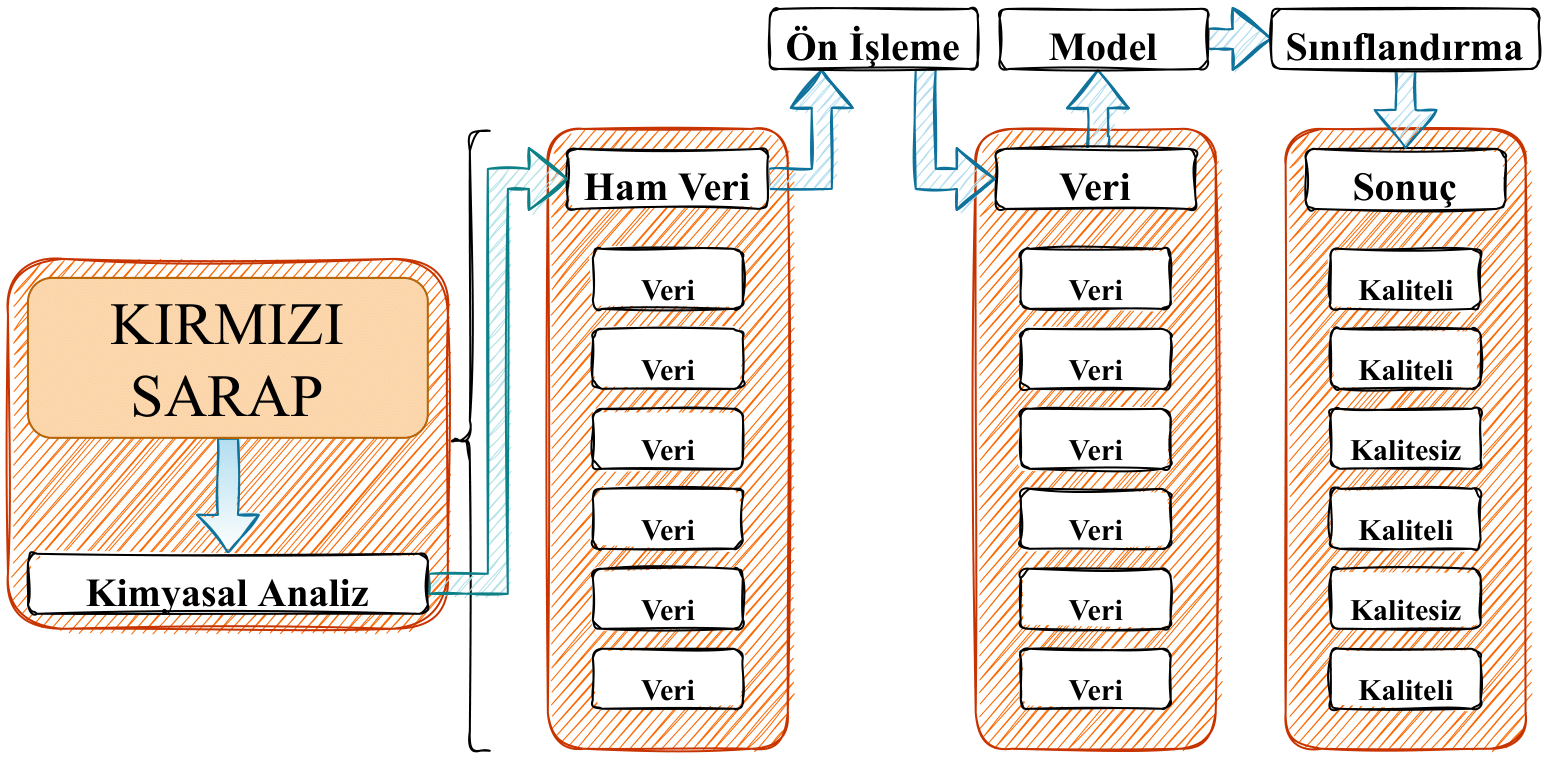
\includegraphics[scale=0.2]{pictures/pic_01.png}&%
		\end{tabular}%
	\end{center}
	\caption{Kırmızı Şarap Kalite Kontrol Süreci}%
	\label{fig:01}
\end{figure}

Projemizin akış diyagramı Şekil \ref{fig:01}'deki gibidir. Makalenin ikinci bölümünde, bahsettiğimiz algortimalar hakkında bilgiler sunulmaktadır. Daha sonraki bölümde ise sonuçlar yer almaktadır.


\section{\textbf{KULLANILAN ALGORİTMALAR}}
\subsection{\textbf{K-Nearest Neighbor}}
\quad Gözetimli (denetimli) öğrenme metotlarından olup  basit sınıflandırma işlemlerinde kullanılır\cite{8}\cite{9}.Sınıflandırma çalışması yaparken elimizdeki veriler hakkında kısıtlı ön bilgiye sahip olduğumuzda tercih etmemiz gereken ilk algoritmalardan biridir\cite{8}.

\begin{figure}[!h]
	\centering%
	%\scriptsize
	\begin{center}
		\begin{tabular}{cc}%
			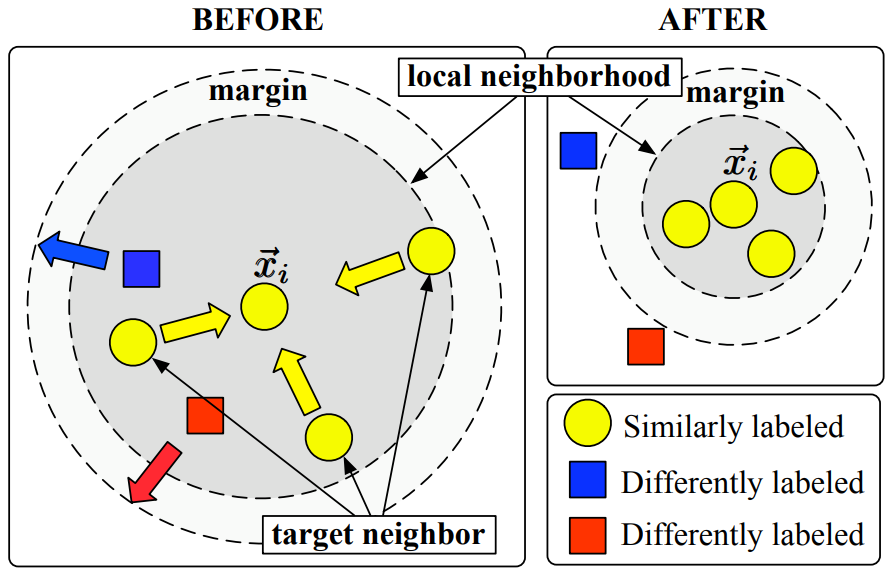
\includegraphics[scale=0.3]{pictures/pic_02.png}&%
		\end{tabular}%
	\end{center}
	\caption{Örnek KNN Şeması\cite{10}}%
	\label{fig:02}
\end{figure}

\quad Bu algoritmanın performansını etkileyen parametreler; uzaklık ölçütü, komşu sayısı(k) ve ağırlıklandırma yöntemidir\cite{7}. Uzaklık ölçütü olarak Manhattan uzaklığı kullandık: \textbf{n} boyutlu düzlemdeki iki konum arasındaki farkların, mutlak değerlerinin toplamıdır. X-Y konumları arasındaki Manhattan uzaklığı: P=(x1, x2,…, xn) ve Q=(y1, y2,…, yn) olmak üzere, Eşitlik \ref{eq:01}'e göre hesaplanır\cite{7}.

\begin{equation}
\label{eq:01}
\Large \sum_{i=1}^{n}\left | x_{i} - y_{i} \right |
\end{equation}

\pagebreak
KNN algoritmasının aşamaları\cite{9}:
\begin{itemize}
\item K değeri belirlenir
\item Diğer konumlara olan uzaklık, Manhattan yöntemiyle hesaplanır
\item Uzaklıklar sıralanarak en yakın komşular bulunur
\item En yakın K adet komşunun kategorileri toplanır
\item Toplam sonucunda ağırlıkta olan kategori seçilerek etiketleme yapılır
\end{itemize}

\subsection{\textbf{Support Vector Machines (SVM)}}
\quad Türkçe adıyla Destek Vektör Makineleri (DVM), istatistiksel öğrenme teorisi geliştiricisi Vapnik tarafından geliştirilmiştir. Sınıflandırma, örüntü tanıma problemleri için kullanılır. Destek Vektör Makineleri, alanındaki birçok tekniğe göre daha yüksek başarı oranına sahiptir. Uygulama sırasında çekirdek fonksiyon seçimi ve parametre optimizasyonu çok önemlidir\cite{11}.

\begin{figure}[!h]
	\centering%
	%\scriptsize
	\begin{center}
		\begin{tabular}{cc}%
			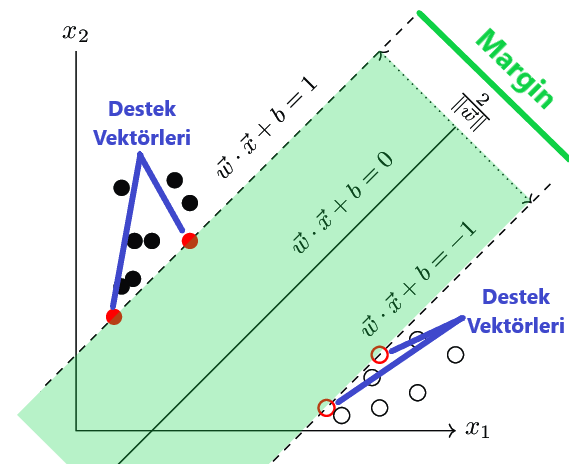
\includegraphics[scale=0.3]{pictures/pic_03.png}&%
		\end{tabular}%
	\end{center}
	\caption{Örnek SVM Şeması\cite{12}}%
	\label{fig:03}
\end{figure}

Şekil \ref{fig:03} üzerinde siyah ve beyaz olmak üzere iki sınıf mevcut. Gelecek verilerin sınıflandırılabilmesi için öncelikle sınıfları birbirinden ayıran bir doğru çizilir. Bu doğrunun -1 ve +1 değerleri arasında kalan yeşil kısım Margin bölgesidir. Margin ne kadar geniş olursa, sınıflar o kadar iyi ayırışıyor demektir. Bu işlemin formülü Eşitlik \ref{eq:02}'deki gibidir.

\begin{equation}
\label{eq:02}
\Large \hat{y}=\left\{\begin{matrix} 0, w^{T} \cdot x + b < 0,\\ 1, w^{T} \cdot x + b \geq 0 \end{matrix}\right.
\end{equation}

\quad Elde ettiğimiz sonuç 0’dan küçük çıkarsa beyaz noktaların bulunduğu kısma yakın olacaktır. Sonuç 0’a eşit veya 0’dan büyük çıkarsa siyah noktaların bulunduğu kısma daha yakın olacaktır\cite{12}.
\pagebreak
\subsection{\textbf{Logistic Regression}}

\quad Lojistik Regresyon,bize sonucu 0 veya 1 şeklinde üreten, değişkenlerin modellenmesinde kullanılan algoritmadır. Örneğin kırmızı şarap kalitesini ele aldığımız zaman; elimizdeki veri setinde 0 kalitesiz, 1 kaliteli durumunu temsil eder. Kısacası Lojistik Regresyon yöntemiyle kullanılan örneklemlerin hangi sınıfa ait olduklarını belirleyebiliriz\cite{13}.

\begin{equation}
\label{eq:03}
\Large f(x)=\frac{1}{1+e^{-z}}
\end{equation}

Lojistik regresyon, $\left(-\infty,+\infty \right)$ aralığındaki değerleri girdi olarak kabul eder\cite{13}.

\begin{figure}[!h]
	\centering%
	%\scriptsize
	\begin{center}
		\begin{tabular}{cc}%
			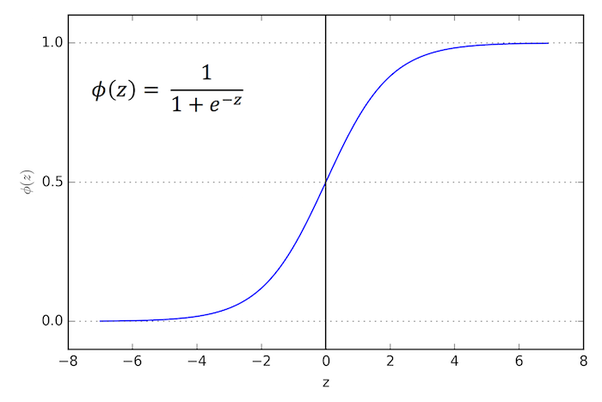
\includegraphics[scale=0.3]{pictures/pic_04.png}&%
		\end{tabular}%
	\end{center}
	\caption{Örnek bir Lojistik Regresyon Şeması\cite{13}}%
	\label{fig:04}
\end{figure}

\subsection{\textbf{Naive Bayes}}
\quad Navie Bayes algoritması sınıflandırıcı teorem olan Bayes’e dayanmaktadır\cite{15}.  Adını ingiliz matematikçi olan Thomas Bayes’ten almıştır\cite{14}. Navie Bayes, elimizdeki örneklerin hangi sınıfa ait olduğunu, işlemler sonucu elde ettiği oranla tahmin eder. Navie Bayes’ın iki önemli kabulü vardır\cite{15}. Bunlar:
\begin{itemize}
\item Elimizde bulunan niteliklerin hepsi aynı derecede önemlidir.
\item Elimizde bulunan nitelikler birbirinden bağımsızdır.
\end{itemize}

\quad Koşullu olasılıklar arasında bağlantı kuran Bayes Teoremi, x özniteliğinin gerçekleşmiş olması durumunda C özniteliğinin gerçekleşmesi veya C özniteliğinin gerçekleşmiş olması durumunda x özniteliğinin gerçekleşmesi durumunu bize verir\cite{15}. Bayes kuralının algoritması Eşitlik \ref{eq:04}'deki gibidir. Eşitlikte yer alan değerler\cite{14}:

\begin{itemize}
\item \textbf{p(x|Cj):} j sınıfından bir örneğin x olma olasılığı
\item \textbf{P(Cj):} j sınıfının ilk olasılığı
\item \textbf{p(x):} Herhangi bir örneğin x olma olasılığı
\item \textbf{P(Cj|x):} x olan bir örneğin j sınıfından olma olasılığı (son olasılık)
\end{itemize}

\begin{equation}
\label{eq:04}
\Large P(C_{j}|x) = \frac {p(x|C_{j}) P(C_{j})} {p(x)} = \frac {p(x|C_{j}) P(C_{j})} {\sum_{k}^{}p(x|C_{k})P(C_{k})}
\end{equation}

\subsection{\textbf{Decision Tree}}
\quad Karar ağaçları, en yaygın kullanılan gözetimli(denetimli) öğrenme algoritmalarından birisidir. Adından da anlaşılacağı üzere ağaç tabanlı öğrenmeye dayalıdır. Tüm problemlere uyarlanabilir\cite{16}. Karar ağacı, kök düğüm değişkeninden başlayarak, ağaç dalı hiyerarşisi gibi dallanır\cite{17}.

\begin{figure}[!h]
	\centering%
	%\scriptsize
	\begin{center}
		\begin{tabular}{cc}%
			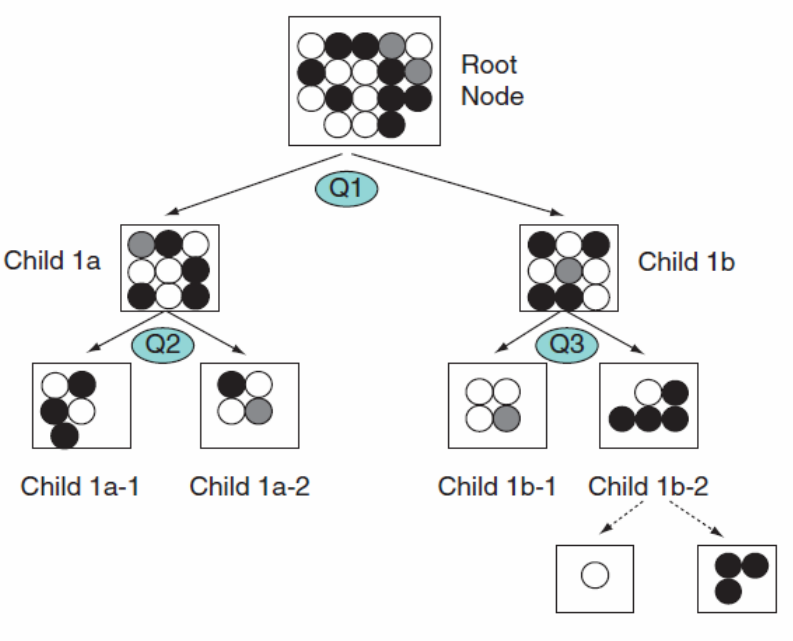
\includegraphics[scale=0.4]{pictures/pic_05.png}&%
		\end{tabular}%
	\end{center}
	\caption{Örnek bir Karar Ağacı Şeması\cite{17}}%
	\label{fig:05}
\end{figure}

\quad Entropi, verilerimizle alakalı belirsizliğin bir ölçüsüdür; dolayısıyla entropinin düşük olması tercih edilir. Sezgisel olarak verilerin tamamı aynı etikete sahipse, veri setinin entropisinin düşük olduğunu söyleyebiliriz\cite{16}.

\begin{equation}
\label{eq:05}
\Large H=-\sum p(x)\log{p(x)}
\end{equation}

\quad Burada; p(x) belirli bir sınıfa ait grubun yüzde oranını, H ise entropiyi belirtmektedir. Karar ağacı, entropiyi en aza indirecek şekilde bölünme yapmalıdır. En iyi bölümlemeyi belirlemek için kullanılan bilgi kazancı, Eşitlik \ref{eq:06}'daki gibi hesaplanır\cite{16}.

\begin{equation}
\label{eq:06}
\Large Gain(S,D) = H(S)-\sum_{V\in D}^{}\frac{\left|V\right|}{\left|S\right|}H(V)
\end{equation}

\quad Burada; \textbf{S} orijinal veri kümesini, \textbf{D} ise kümenin bölünmüş bir parçasını temsil eder. Her \textbf{V} değeri, \textbf{S}'nin alt kümesidir\cite{16}.
\pagebreak
\subsection{\textbf{Bagging}}
\quad Türkçe adıyla torbalama yöntemi olarak adlandırılan Bagging algoritması 1996 yılında Breiman tarafından geliştirilmiştir. Bagging (torbalama) algoritmasının çalışma biçimi Şekil \ref{fig:06}'da belirtilmiştir. Şekil \ref{fig:06}'daki aşamaların açıklamaları\cite{18}:

\begin{itemize}
\item \textbf{Bootstrap sampling:} Orijinal veri kümesi, alt kümelere bölünür.
\item \textbf{Model training:} Bu alt kümelerin her birinde ayrı ayrı temel (zayıf) model oluşturulur.
\item \textbf{Model forecasting:} Modeller birbirinden bağımsız ancak paralel olarak çalışır.
\item \textbf{Result aggregating:} Tüm modellerin tahmin sonuçları birleştirilerek niai tahmin belirlenir.
\end{itemize}

\begin{figure}[!h]
	\centering%
	%\scriptsize
	\begin{center}
		\begin{tabular}{cc}%
			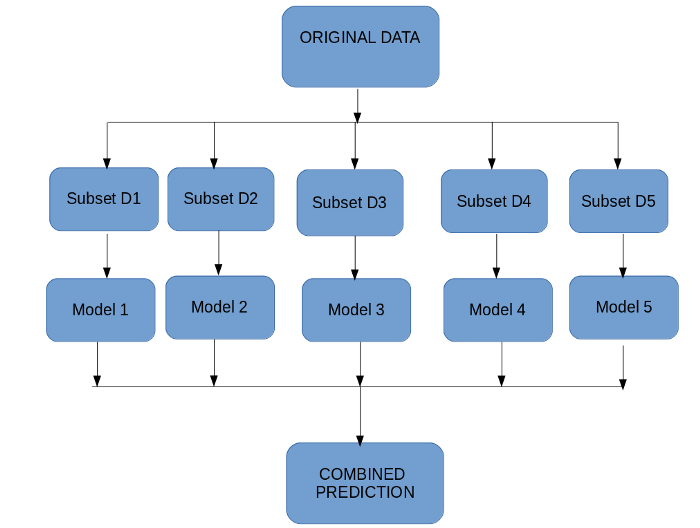
\includegraphics[scale=0.35]{pictures/pic_06.png}&%
		\end{tabular}%
	\end{center}
	\caption{Örnek bir Torbalama Şeması\cite{18}}%
	\label{fig:06}
\end{figure}
\newpage
\subsection{\textbf{Random Forest Tree}}
\quad Türkçe adıyla Rastgele Orman Ağacı Algoritması, denetimli bir sınıflandırma algoritmasıdır. Adından da anlaşılacağı gibi, algoritmamız rastgele bir orman yaratıyor. Bu ormandaki ağaç sayısı ve elde edilebilecek sonuçlar arasında doğrusal bir ilişki vardır. Ağaç sayısı arttıkça elde edilecek olan sonucun kesinliği de artar. Rastgele Orman Ağacı’nın Karar Ağacı’ndan farkı; kök bulma ve düğümleri bölme işlemlerinin çalışıyor olmasıdır\cite{19}. Rastgele Orman Ağacı’nın şeması Şekil \ref{fig:07}'de verilmiştir.

\begin{figure}[!h]
	\centering%
	%\scriptsize
	\begin{center}
		\begin{tabular}{cc}%
			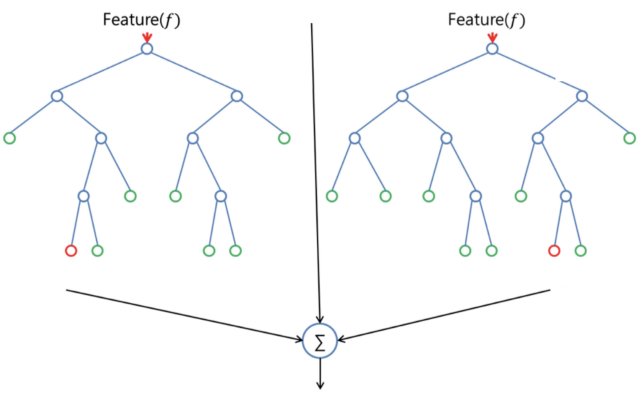
\includegraphics[scale=0.29]{pictures/pic_07.png}&%
		\end{tabular}%
	\end{center}
	\caption{Örnek bir Rastgele Orman Ağacı Şeması\cite{20}}%
	\label{fig:07}
\end{figure}

\quad Rastgele Orman Ağacı, kullanıcıdan iki parametre alır: m parametresi en iyi bölünmeyi belirlemek için her düğümde kullanılan değişkenlerin sayısı, N geliştirilecek ağaç sayısı. Öncelikle eğitim verilerinin 2/3'ü kullanılarak önyükleme örnekleri oluşturulur. Geri kalan 1/3'lük kısım (OOB: out of bag) ise hataları test etmek için kullanılır\cite{21}.

\quad Her bir düğümde \textbf{m} değişkenleri, tüm değişkenlerin arasından rastgele seçilerek en iyi dal belirlenir. \textbf{M} adet değişkenin kareköküne eşit olarak alınan \textbf{m} değişken, genellikle optimuma en yakın sonucu verir\cite{21}.

\quad Sınıfların homojenliği $Gini$ indexi hesaplanarak ölçülür. $Gini$ indexi ne kadar düşükse, sınıf da o kadar homojendir. Bir düğümün alt $Gini$ indexi üst $Gini$ indexinden daha az olduğu durumlarda incelenen dal başarılı sayılır\cite{21}. $Gini$ indexinin formülü Eşitlik \ref{eq:07}'de verilmiştir. Formül değişkenlerinin temsil ettiği veriler de aşağıdaki gibidir;

\begin{itemize}
\item \textbf{T:} Tüm veri seti
\item \textbf{pj:} Veri setindeki her bir verinin kendinden küçük ve kendünden büyük eleman sayılarına bölümü
\item \textbf{n:} Seçilen verimiz
\end{itemize}

\begin{equation}
\label{eq:07}
\Large Gini(T)=1-\sum_{j=1}^{n}(p_{j})^{2}
\end{equation}

\pagebreak
\section{\textbf{DENEYSEL SONUÇLAR VE TARTIŞMA}}

\subsection{\textbf{K-Nearest Neighbor}}
Şekil \ref{fig:08}'de \textbf{K-Nearest Neighbor} algoritmamızın hata matrisinin görselini görüyoruz. Hata matrisindeki değerleri kullanarak:
\linebreak \textbf{Doğruluk değeri: } $(145 + 154) / (145 + 68 + 113 + 154) = 0.62$
\linebreak \textbf{Hata oranı: } $1 - Dogruluk Degeri(0.62) = 0.38$

\begin{figure}[!h]
	\centering%
	%\scriptsize
	\begin{center}
		\begin{tabular}{cc}%
			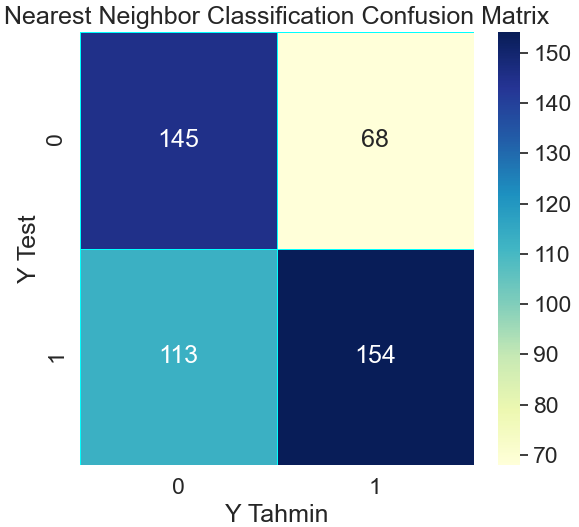
\includegraphics[scale=0.5]{pictures/pic_08.png}&%
		\end{tabular}%
	\end{center}
	\caption{K-Nearest Neighbor Hata Matrisi}%
	\label{fig:08}
\end{figure}

\quad \textbf{K-Nearest Neighbor} algoritmasını Cross-Validation'a soktuk ve 30 kere rastgele verilerle çalışmasını sağladık. Bu değerlerin grafiği Şekil \ref{fig:09}'daki gibidir. Şekildeki değerlerin ortalaması 0.6289, standart devinasyonu ise 0.1050'dir. 

\begin{figure}[!h]
	\centering%
	%\scriptsize
	\begin{center}
		\begin{tabular}{cc}%
			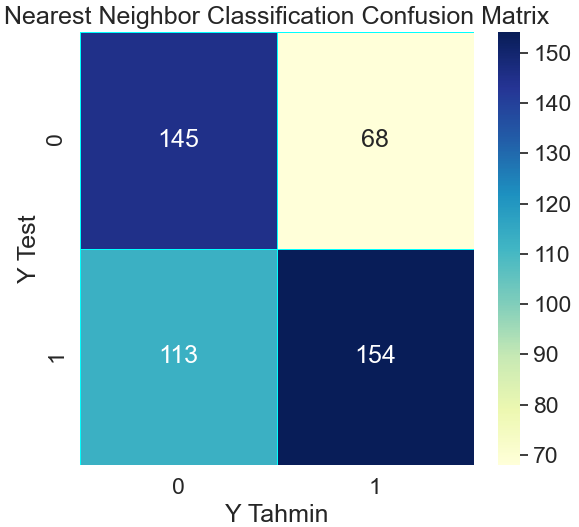
\includegraphics[scale=0.2]{pictures/pic_09.png}&%
		\end{tabular}%
	\end{center}
	\caption{{K-Nearest Neighbor Cross-Validation Değerleri}}%
	\label{fig:09}
\end{figure}

\pagebreak
\subsection{\textbf{Support Vector Machines (SVM)}}
Şekil \ref{fig:10}'da \textbf{Support Vector Machines} algoritmamızın hata matrisinin görselini görüyoruz. Hata matrisindeki değerleri kullanarak:
\linebreak \textbf{Doğruluk değeri: } $(145 + 187) / (145 + 68 + 80 + 187) = 0.69$
\linebreak \textbf{Hata oranı: } $1 - Dogruluk Degeri(0.69) = 0.31$
\begin{figure}[!h]
	\centering%
	%\scriptsize
	\begin{center}
		\begin{tabular}{cc}%
			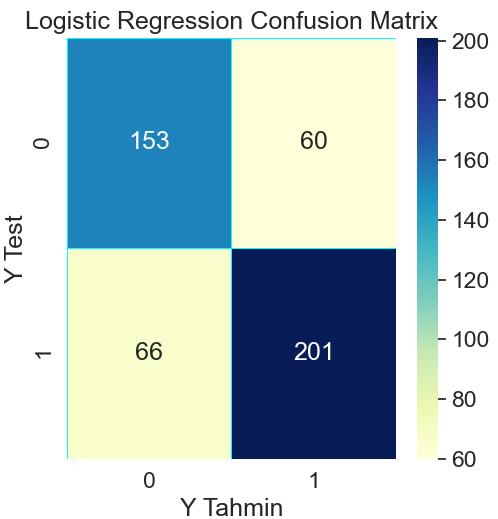
\includegraphics[scale=0.5]{pictures/pic_10.png}&%
		\end{tabular}%
	\end{center}
	\caption{{Support Vector Machines Hata Matrisi}}%
	\label{fig:10}
\end{figure}

\quad \textbf{Support Vector Machines} algoritmasını Cross-Validation'a soktuk ve 30 kere rastgele verilerle çalışmasını sağladık. Bu değerlerin grafiği Şekil \ref{fig:11}'deki gibidir. Şekildeki değerlerin ortalaması 0.7179, standart devinasyonu ise 0.1032'dir. 

\begin{figure}[!h]
	\centering%
	%\scriptsize
	\begin{center}
		\begin{tabular}{cc}%
			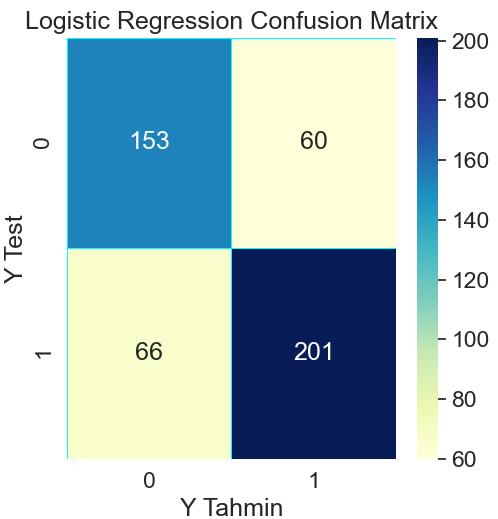
\includegraphics[scale=0.2]{pictures/pic_11.png}&%
		\end{tabular}%
	\end{center}
	\caption{{Support Vector Machines Cross-Validation Değerleri}}%
	\label{fig:11}
\end{figure}

\pagebreak
\subsection{\textbf{Logistic Regression}}
Şekil \ref{fig:12}'de \textbf{Logistic Regression} algoritmamızın hata matrisinin görselini görüyoruz. Hata matrisindeki değerleri kullanarak:
\linebreak \textbf{Doğruluk değeri: } $(153 + 201) / (153 + 60 + 66 + 201) = 0.73$
\linebreak \textbf{Hata oranı: } $1 - Dogruluk Degeri(0.73) = 0.27$
\begin{figure}[!h]
	\centering%
	%\scriptsize
	\begin{center}
		\begin{tabular}{cc}%
			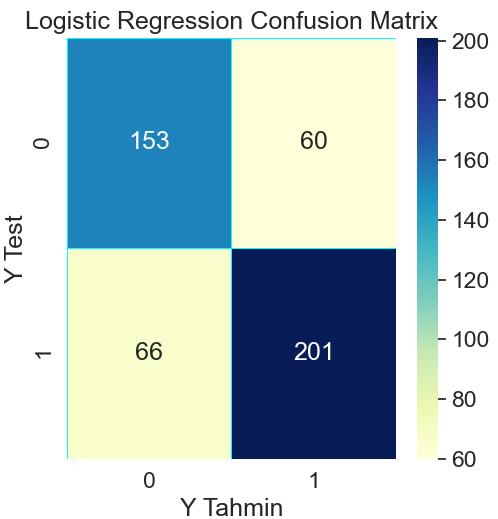
\includegraphics[scale=0.5]{pictures/pic_12.png}&%
		\end{tabular}%
	\end{center}
	\caption{{Logistic Regression Hata Matrisi}}%
	\label{fig:12}
\end{figure}

\quad \textbf{Logistic Regression} algoritmasını Cross-Validation'a soktuk ve 30 kere rastgele verilerle çalışmasını sağladık. Bu değerlerin grafiği Şekil \ref{fig:13}'deki gibidir. Şekildeki değerlerin ortalaması 0.7348, standart devinasyonu ise 0.0932'dir. 

\begin{figure}[!h]
	\centering%
	%\scriptsize
	\begin{center}
		\begin{tabular}{cc}%
			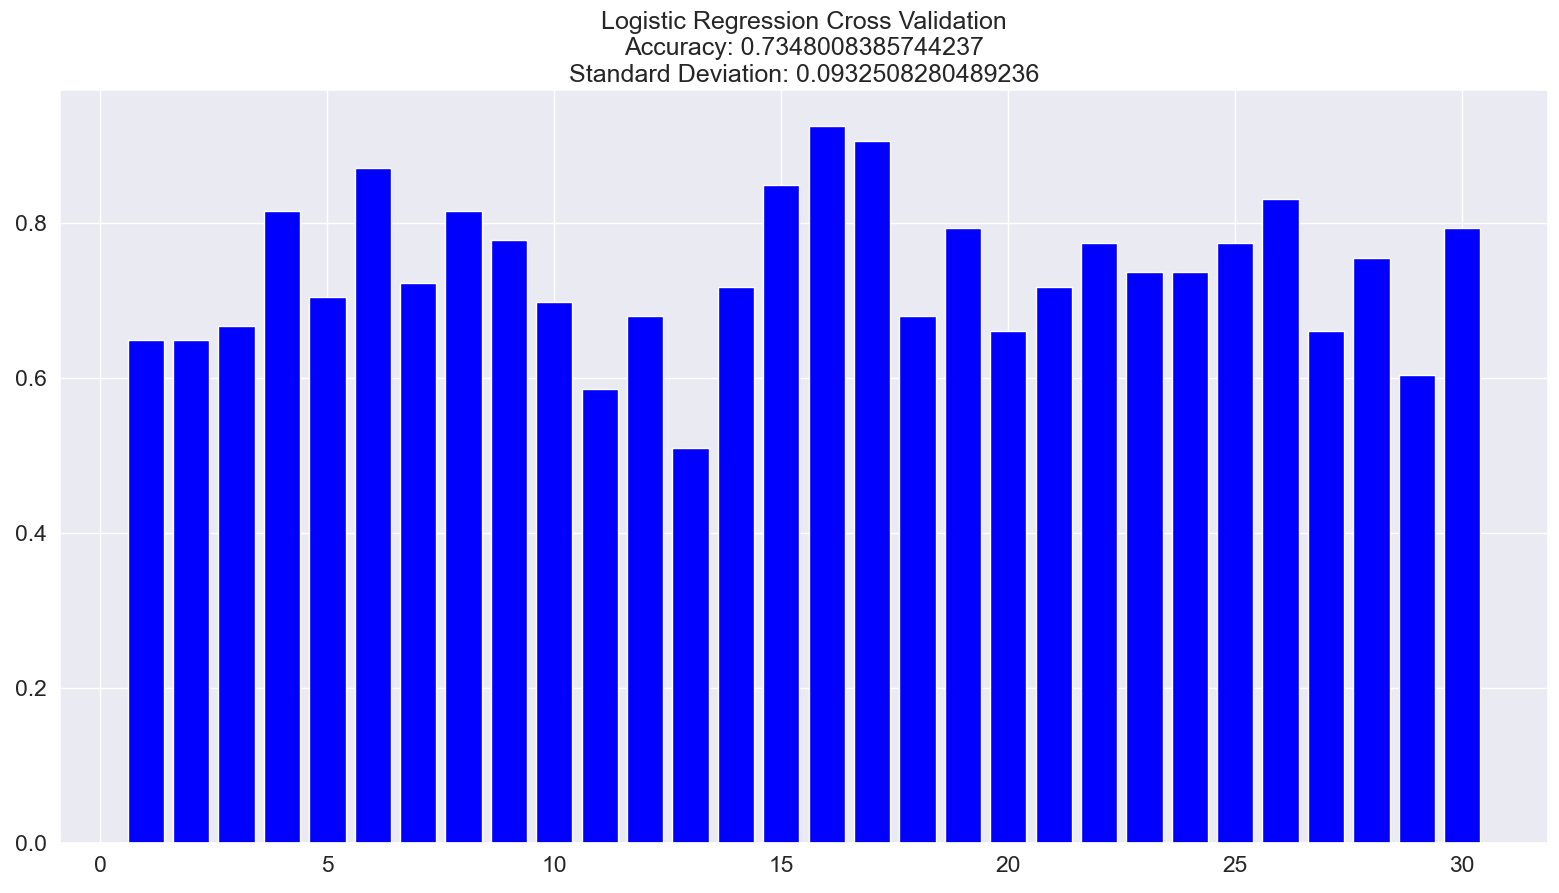
\includegraphics[scale=0.2]{pictures/pic_13.png}&%
		\end{tabular}%
	\end{center}
	\caption{{Logistic Regression Cross-Validation Değerleri}}%
	\label{fig:13}
\end{figure}

\pagebreak
\subsection{\textbf{Naive Bayes}}
Şekil \ref{fig:14}'de \textbf{Naive Bayes} algoritmamızın hata matrisinin görselini görüyoruz. Hata matrisindeki değerleri kullanarak:
\linebreak \textbf{Doğruluk değeri: } $(150 + 209) / (150 + 63 + 58 + 209) = 0.74$
\linebreak \textbf{Hata oranı: } $1 - Dogruluk Degeri(0.73) = 0.26$
\begin{figure}[!h]
	\centering%
	%\scriptsize
	\begin{center}
		\begin{tabular}{cc}%
			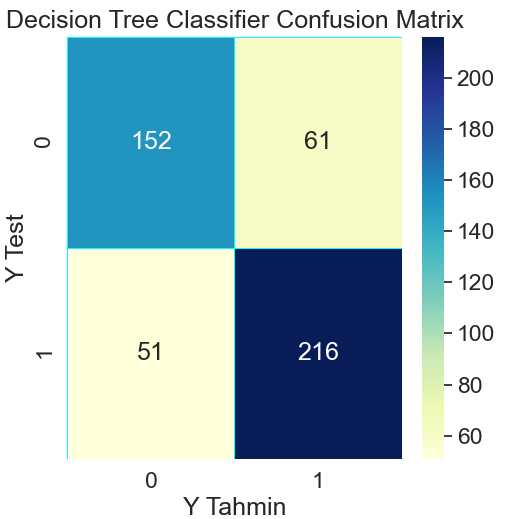
\includegraphics[scale=0.5]{pictures/pic_14.png}&%
		\end{tabular}%
	\end{center}
	\caption{{Naive Bayes Hata Matrisi}}%
	\label{fig:14}
\end{figure}

\quad \textbf{Naive Bayes} algoritmasını Cross-Validation'a soktuk ve 30 kere rastgele verilerle çalışmasını sağladık. Bu değerlerin grafiği Şekil \ref{fig:15}'deki gibidir. Şekildeki değerlerin ortalaması 0.7222, standart devinasyonu ise 0.1130'dur. 

\begin{figure}[!h]
	\centering%
	%\scriptsize
	\begin{center}
		\begin{tabular}{cc}%
			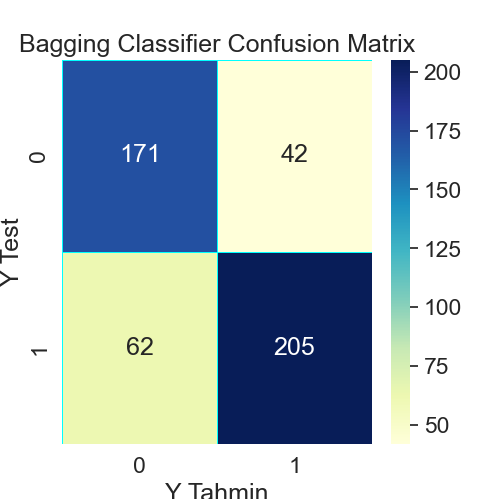
\includegraphics[scale=0.2]{pictures/pic_15.png}&%
		\end{tabular}%
	\end{center}
	\caption{{Naive Bayes Cross-Validation Değerleri}}%
	\label{fig:15}
\end{figure}

\pagebreak
\subsection{\textbf{Decision Tree}}
Şekil \ref{fig:16}'da \textbf{Decision Tree} algoritmamızın hata matrisinin görselini görüyoruz. Hata matrisindeki değerleri kullanarak:
\linebreak \textbf{Doğruluk değeri: } $(152 + 216) / (152 + 61 + 51 + 216) = 0.76$
\linebreak \textbf{Hata oranı: } $1 - Dogruluk Degeri(0.76) = 0.24$
\begin{figure}[!h]
	\centering%
	%\scriptsize
	\begin{center}
		\begin{tabular}{cc}%
			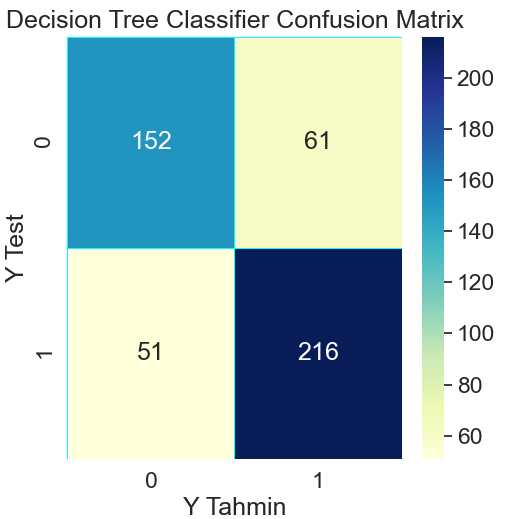
\includegraphics[scale=0.5]{pictures/pic_16.png}&%
		\end{tabular}%
	\end{center}
	\caption{{Decision Tree Hata Matrisi}}%
	\label{fig:16}
\end{figure}

\quad \textbf{Decision Tree} algoritmasını Cross-Validation'a soktuk ve 30 kere rastgele verilerle çalışmasını sağladık. Bu değerlerin grafiği Şekil \ref{fig:17}'deki gibidir. Şekildeki değerlerin ortalaması 0.6879, standart devinasyonu ise 0.0903'dur. 

\begin{figure}[!h]
	\centering%
	%\scriptsize
	\begin{center}
		\begin{tabular}{cc}%
			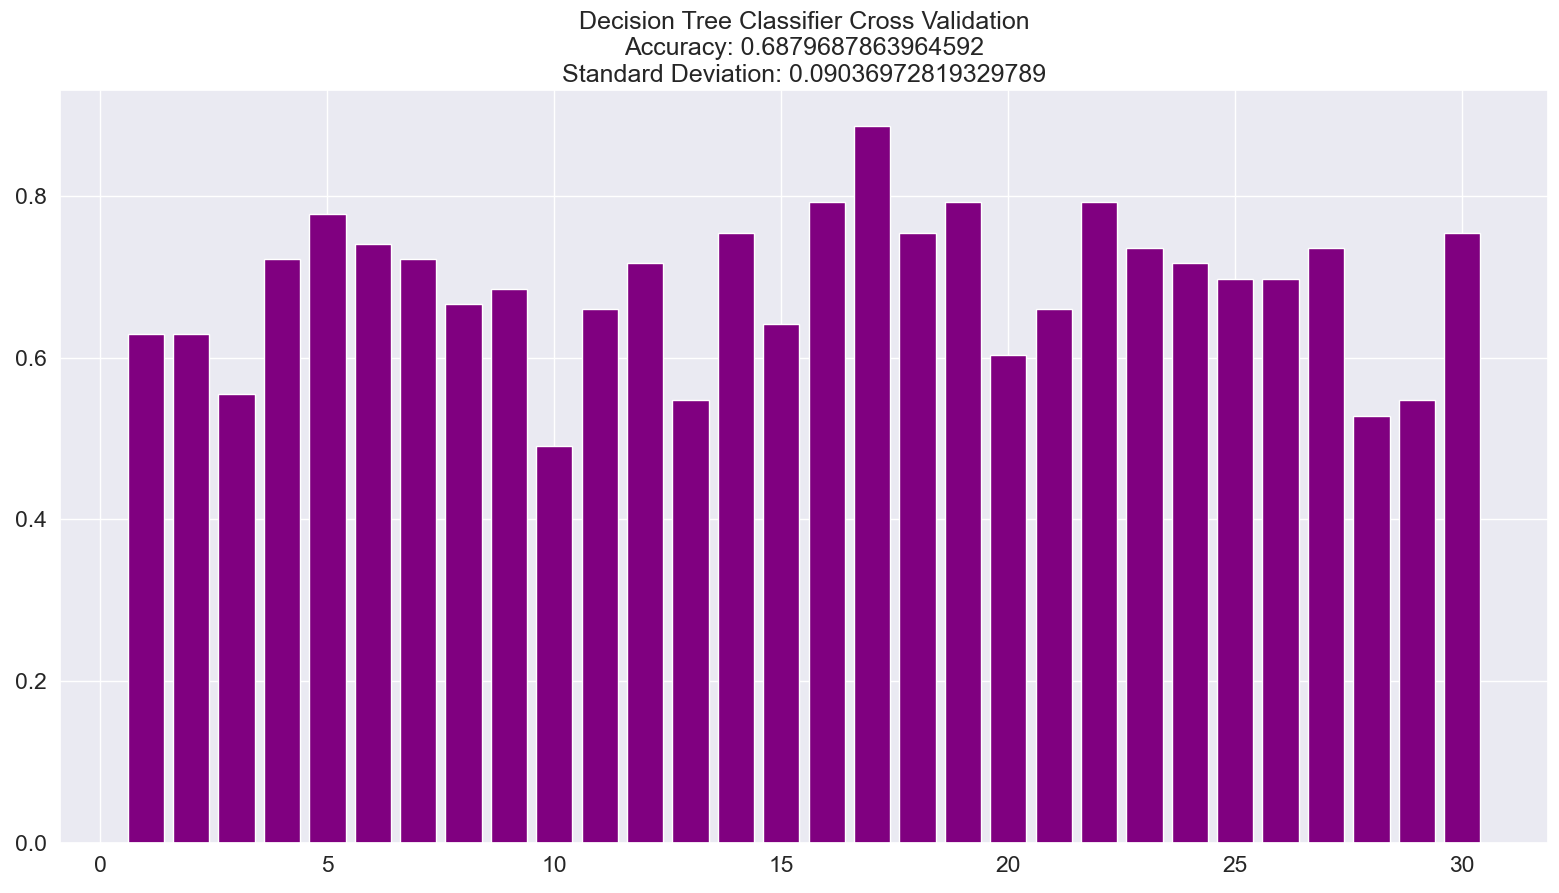
\includegraphics[scale=0.2]{pictures/pic_17.png}&%
		\end{tabular}%
	\end{center}
	\caption{{Decision Tree Cross-Validation Değerleri}}%
	\label{fig:17}
\end{figure}

\pagebreak
\subsection{\textbf{Bagging}}
Şekil \ref{fig:18}'de \textbf{Bagging} algoritmamızın hata matrisinin görselini görüyoruz. Hata matrisindeki değerleri kullanarak:
\linebreak \textbf{Doğruluk değeri: } $(172 + 205) / (172 + 41 + 62 + 205) = 0.78$
\linebreak \textbf{Hata oranı: } $1 - Dogruluk Degeri(0.78) = 0.22$
\begin{figure}[!h]
	\centering%
	%\scriptsize
	\begin{center}
		\begin{tabular}{cc}%
			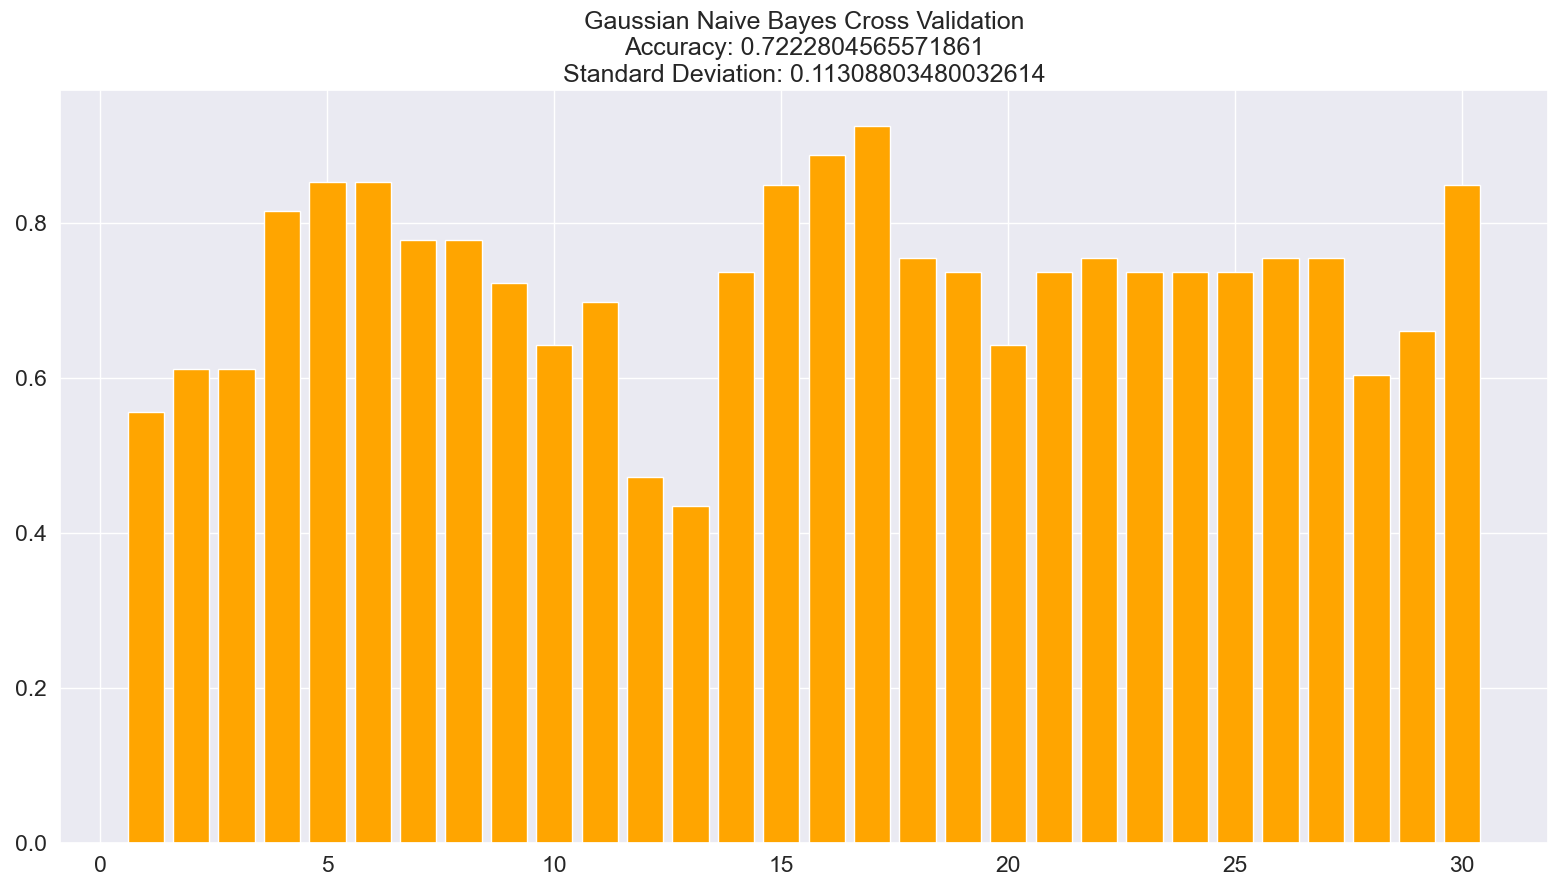
\includegraphics[scale=0.5]{pictures/pic_18.png}&%
		\end{tabular}%
	\end{center}
	\caption{{Bagging Hata Matrisi}}%
	\label{fig:18}
\end{figure}

\quad \textbf{Bagging} algoritmasını Cross-Validation'a soktuk ve 30 kere rastgele verilerle çalışmasını sağladık. Bu değerlerin grafiği Şekil \ref{fig:19}'daki gibidir. Şekildeki değerlerin ortalaması 0.6986, standart devinasyonu ise 0.0955'dur. 

\begin{figure}[!h]
	\centering%
	%\scriptsize
	\begin{center}
		\begin{tabular}{cc}%
			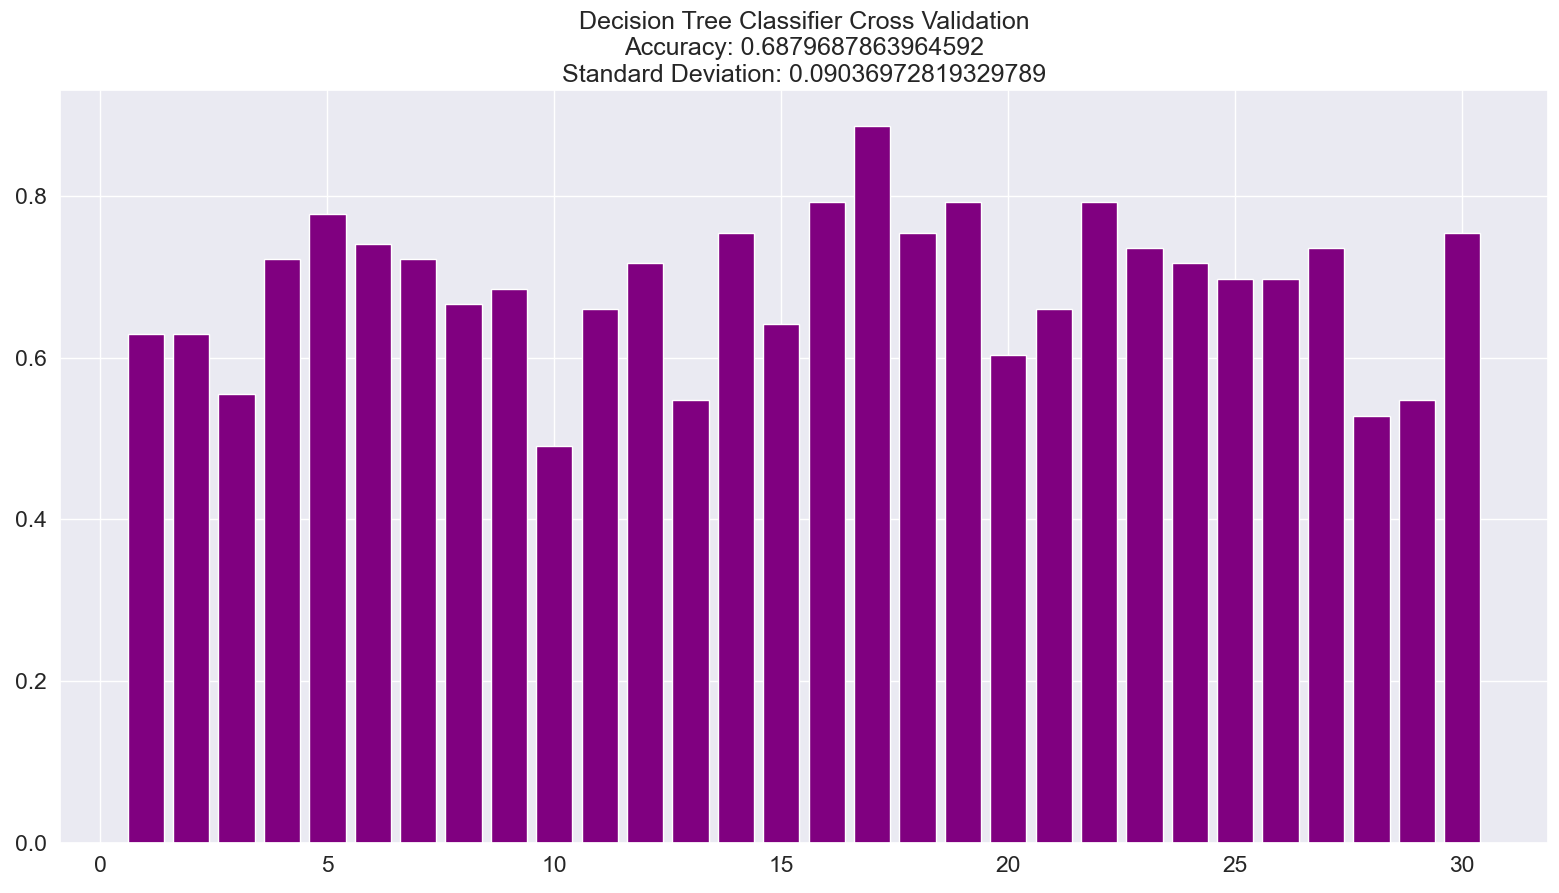
\includegraphics[scale=0.2]{pictures/pic_19.png}&%
		\end{tabular}%
	\end{center}
	\caption{{Bagging Cross-Validation Değerleri}}%
	\label{fig:19}
\end{figure}

\pagebreak
\subsection{\textbf{Random Forest Tree}}
Şekil \ref{fig:20}'de \textbf{Random Forest Tree} algoritmamızın hata matrisinin görselini görüyoruz. Hata matrisindeki değerleri kullanarak:
\linebreak \textbf{Doğruluk değeri: } $(164 + 221) / (164 + 49 + 46 + 221) = 0.80$
\linebreak \textbf{Hata oranı: } $1 - Dogruluk Degeri(0.80) = 0.20$
\begin{figure}[!h]
	\centering%
	%\scriptsize
	\begin{center}
		\begin{tabular}{cc}%
			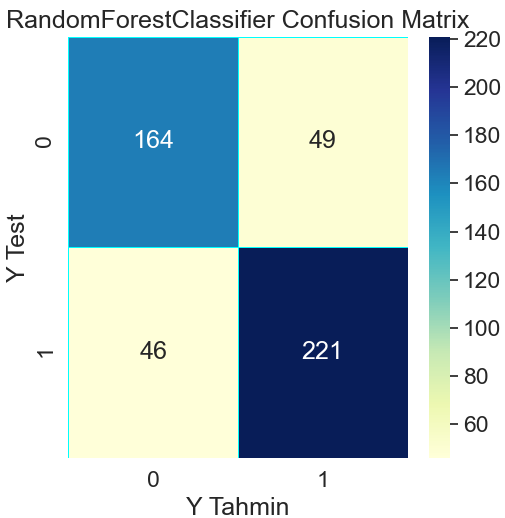
\includegraphics[scale=0.5]{pictures/pic_20.png}&%
		\end{tabular}%
	\end{center}
	\caption{{Random Forest Tree Hata Matrisi}}%
	\label{fig:20}
\end{figure}

\quad \textbf{Random Forest Tree} algoritmasını Cross-Validation'a soktuk ve 30 kere rastgele verilerle çalışmasını sağladık. Bu değerlerin grafiği Şekil \ref{fig:21}'deki gibidir. Şekildeki değerlerin ortalaması 0.7448, standart devinasyonu ise 0.1085'dur. 

\begin{figure}[!h]
	\centering%
	%\scriptsize
	\begin{center}
		\begin{tabular}{cc}%
			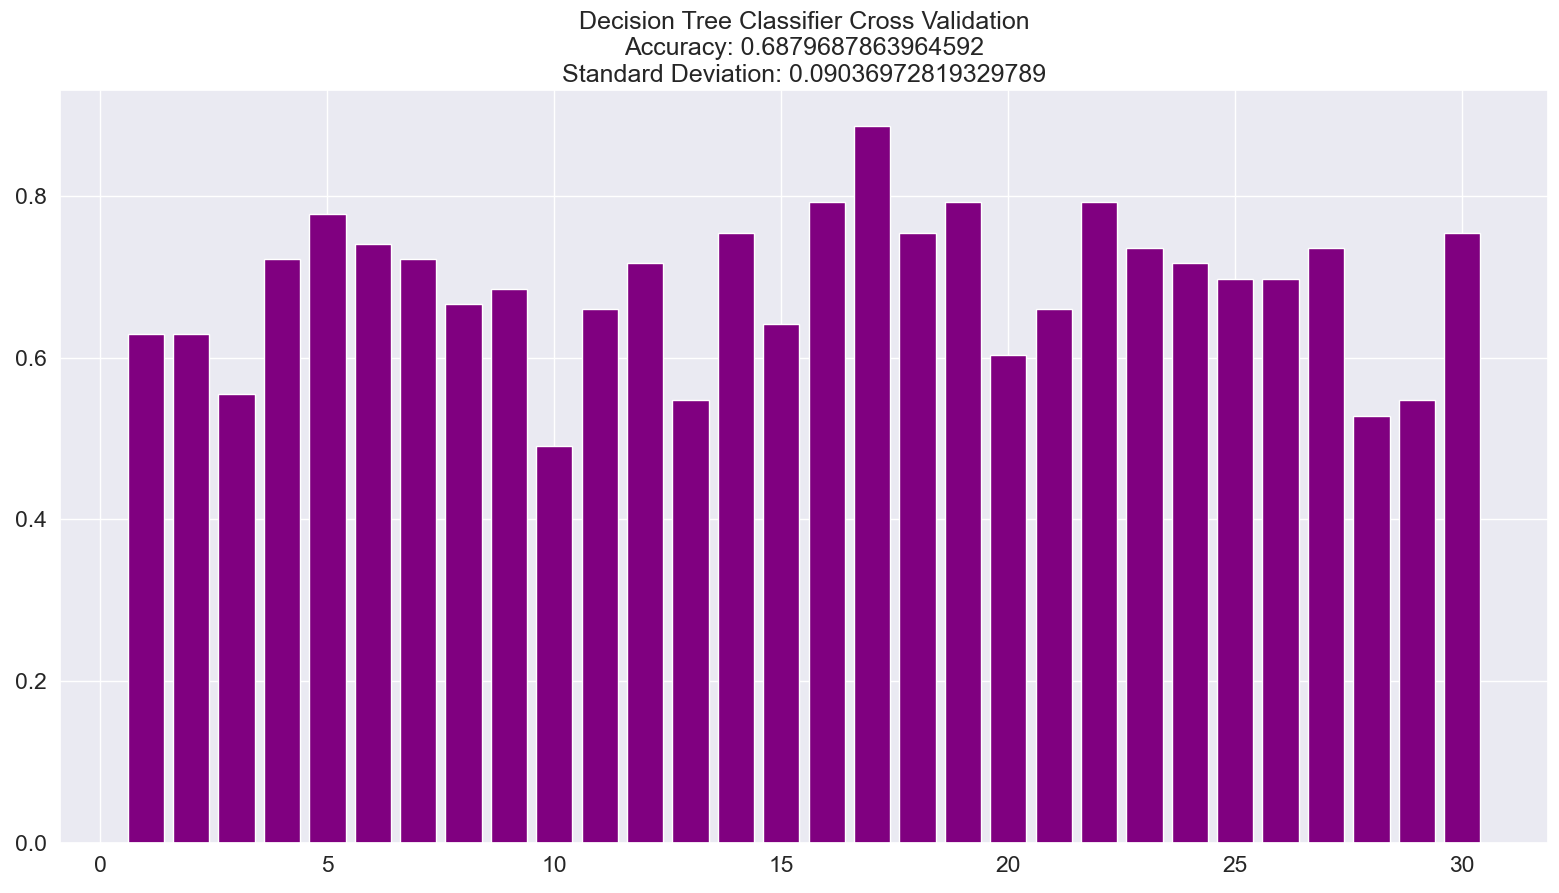
\includegraphics[scale=0.2]{pictures/pic_21.png}&%
		\end{tabular}%
	\end{center}
	\caption{{Random Forest Tree Cross-Validation Değerleri}}%
	\label{fig:21}
\end{figure}

\pagebreak
\subsection{\textbf{Tüm Algoritmalara Ait Sonuçlar \& ROC Eğrisi Grafiği}}
\quad Belirlediğimiz algoritmaları çalıştırdık ve sonuçlarını aldık. Bu sonuçları görsel olarak Şekil \ref{fig:22}'de belirttik. Sonuçlar liste olarak:

\textbf{Nearest Neighbor Classification = Kırmızı}
\begin{itemize}
\item \quad Doğruluk: 0.62
\item \quad MSE: 0.37
\end{itemize}

\textbf{C-Support Vector Classification = Gri}
\begin{itemize}
\item \quad Doğruluk: 0.69
\item \quad MSE: 0.30
\end{itemize}

\textbf{Logistic Regression = Mavi}
\begin{itemize}
\item \quad Doğruluk: 0.73
\item \quad MSE: 0.26
\end{itemize}

\textbf{Gaussian Naive Bayes = Turuncu}
\begin{itemize}
\item \quad Doğruluk: 0.74
\item \quad MSE: 0.25
\end{itemize}

\textbf{Decision Tree Classifier = Mor}
\begin{itemize}
\item \quad Doğruluk: 0.76
\item \quad MSE: 0.23
\end{itemize}

\textbf{Bagging Classifier = Sarı}
\begin{itemize}
\item \quad Doğruluk: 0.78
\item \quad MSE: 0.21
\end{itemize}

\textbf{RandomForestClassifier = Pembe}
\begin{itemize}
\item \quad Doğruluk: 0.80
\item \quad MSE: 0.19
\end{itemize}

\begin{figure}[!h]
	\centering%
	%\scriptsize
	\begin{center}
		\begin{tabular}{cc}%
			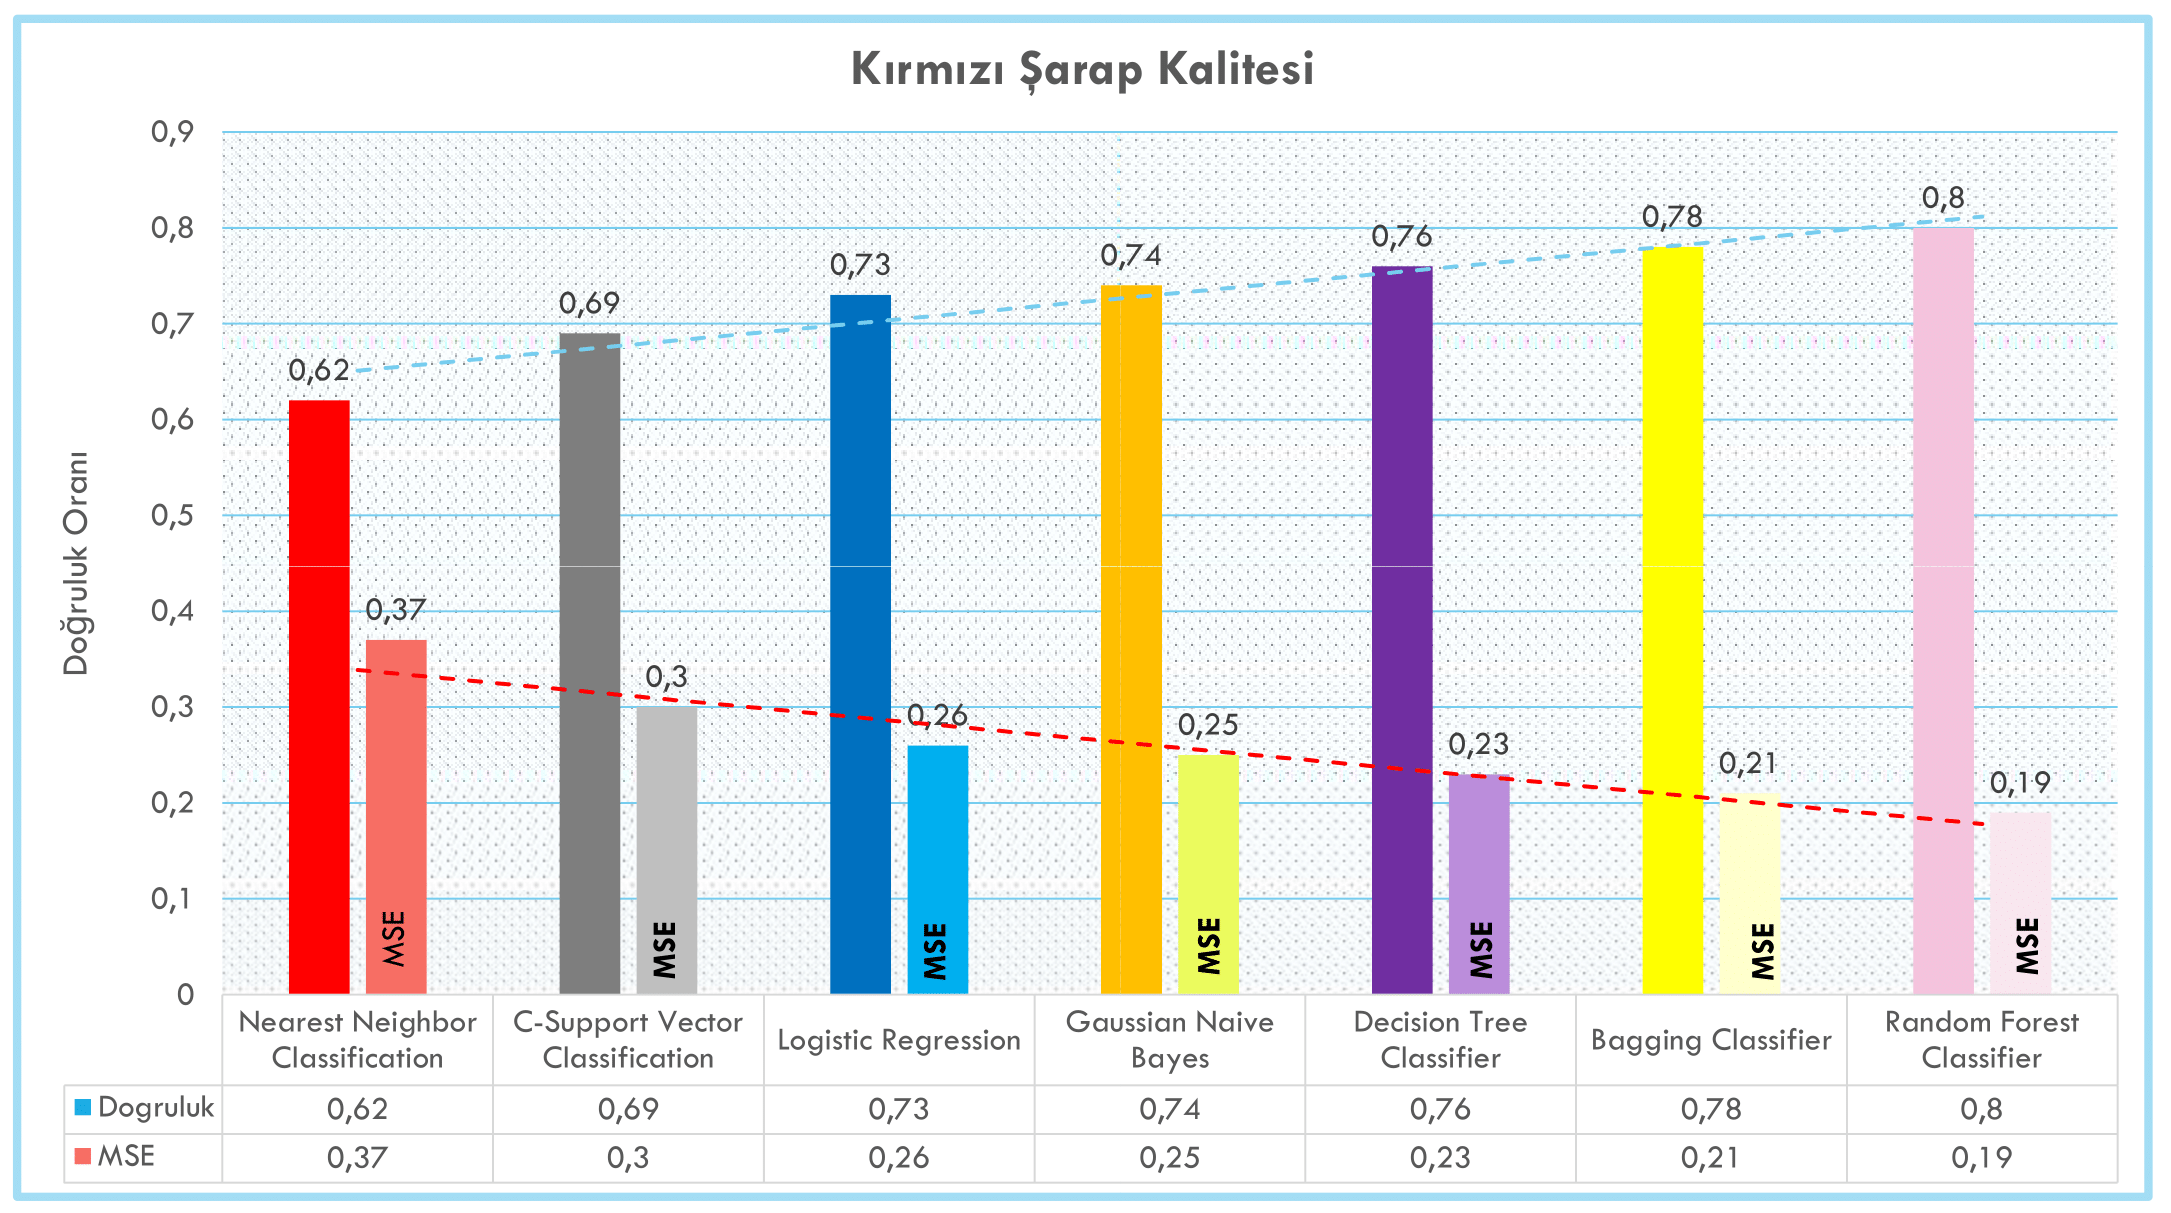
\includegraphics[scale=0.15]{pictures/pic_22.png}&%
		\end{tabular}%
	\end{center}
	\caption{Tüm Algoritmaların Doğruluk \& MSE Oranları}%
	\label{fig:22}
\end{figure}
\pagebreak

\quad Makine öğrenmesinde performans ölçümünde ROC eğrisinden yararlanırız. Bu eğrilerin AUC(doğruluk) değerleri de mevcuttur ancak algoritmanın tahmin doğruluk skoruyla karıştırılmamalıdır\cite{22}. Elimizdeki algoritmaların ROC eğrilerini Şekil \ref{fig:23}'de belirttik. Eğrilerin doğruluk oranları da listedeki gibidir:
\begin{itemize}
\item \textbf{Nearest Neighbor Classification}: 0.62
\item \textbf{C-Support Vector Classification}: 0.69
\item \textbf{Logistic Regression}: 0.73
\item \textbf{Gaussian Naive Bayes}: 0.74
\item \textbf{Decision Tree Classifier}: 0.76
\item \textbf{Bagging Classifier}: 0.78
\item \textbf{RandomForestClassifier}: 0.79
\end{itemize}

\begin{figure}[!h]
	\centering%
	%\scriptsize
	\begin{center}
		\begin{tabular}{cc}%
			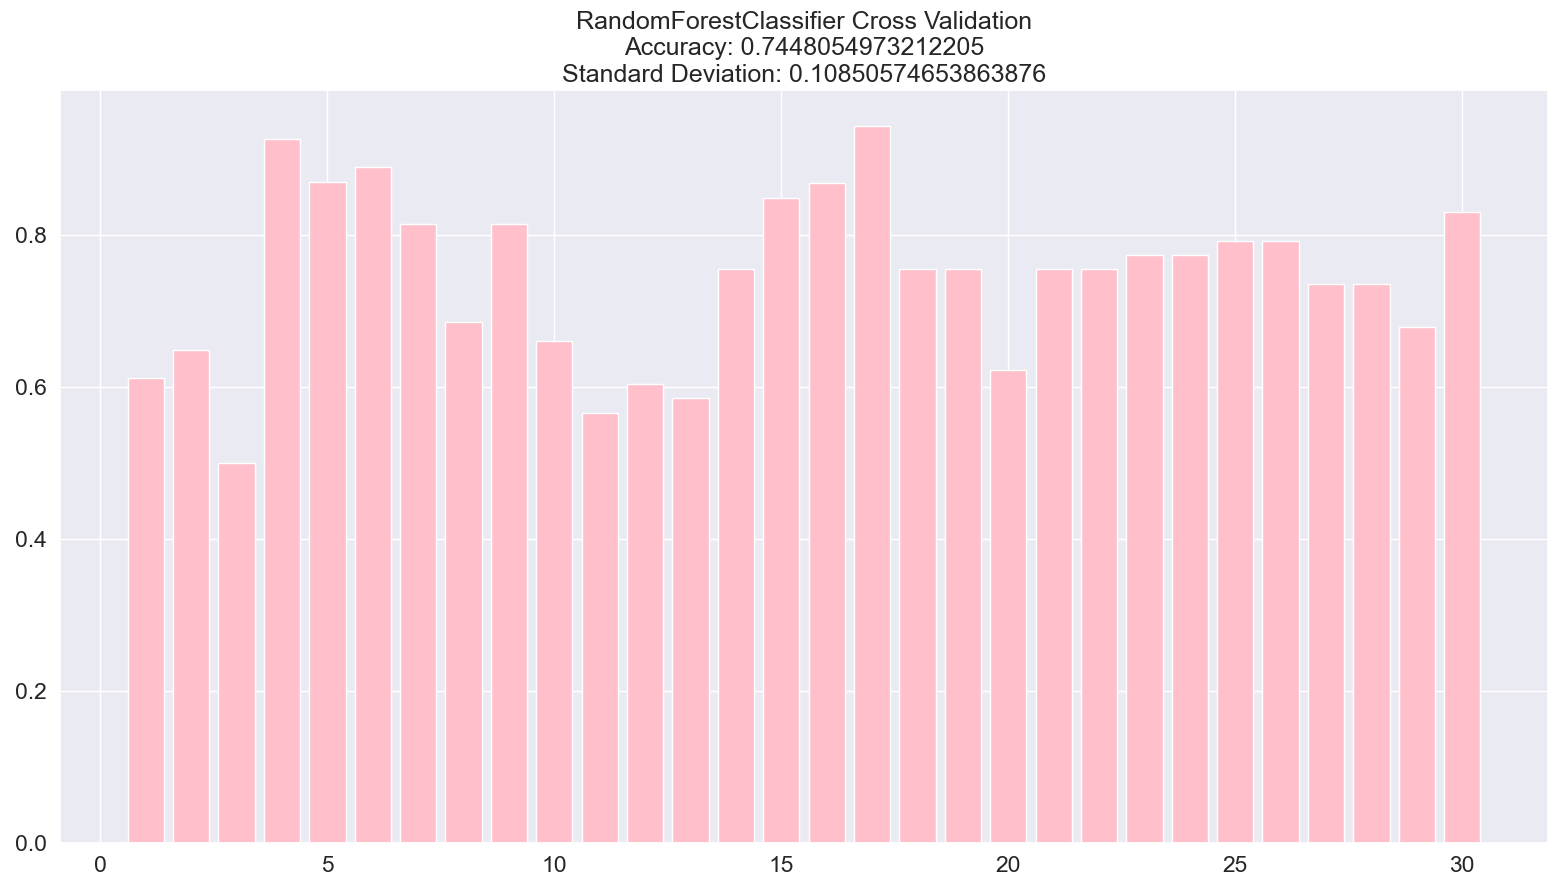
\includegraphics[scale=0.6]{pictures/pic_23.png}&%
		\end{tabular}%
	\end{center}
	\caption{Tüm Algoritmaların ROC Eğrileri ve AUC Değerleri}%
	\label{fig:23}
\end{figure}

\quad Kullandığımız algoritmalardan en başarılı olan Random Forest Tree algoritması oldu. \%80 lik doğruluk oranıyla diğer algoritmaları geride bıraktı. Ortalama hata karesi değeri diğer algoritmalara göre daha düşük (0.19) çıktı. En düşük başarıya sahip olan algoritmamız ise \%62'lik başarı oranıyla K-Nearest Neighbor algoritması oldu. Ortalama hata karesi değerini de Random Forest Tree'ninkine göre yüksek kalan 0.37 olarak elde ettik. Algoritmaların bu değerlerini Şekil \ref{fig:22}'de belirttik. Diğer algoritmalar ise birbirine oldukça yakın değerler verdi. Bagging algoritması ise \%78 doğruluk oranı verirken 0.21 MSE değeriyle, en verimli ikinci algoritma oldu. Kullandığımız en verimli üçüncü algoritma ise \%76 doğruluk değeriyle Decision Tree algoritması oldu. MSE değeri olarak da 0.23 verdi. Decision Tree'nin ardından gelen algoritma ise Naive Bayes algoritması oldu. \%74 doğruluk değerine ve 0.25 MSE değerine sahip bir şekilde Logistic Regression'u geride bıraktı. Logistic Regression ise \%73 doğruluk oranıyla birlikte 0.26 MSE değerini alarak en verimli beşinci algoritma oldu. Elimizdeki verimlilik düzeyi en düşük olan K-Nearest Neighbor algoritması ile Logistic Regression arasında kalan tek algoritma ise C-Support Vector algoritması. Bu algoritmanın doğruluk değeri \%69'ken MSE değeri de 0.3 olarak elimize geçti.

\section{\textbf{SONUÇ}}
\quad Bu projede kullanılan veri seti sayesinde kırmızı şarabın kalitesinin, ortalamanın üstünde veya altında olduğunu tahmin etmeye çalıştık. Bunu yapmak için, önceden belirlediğimiz algoritmaları kullandık ve sonuçlarını karşılaştırdık. Her algoritmada farklı doğruluk değerleri elde ettik. Bazı algoritmalar bu veri seti için daha yeterli olurken bazıları daha yetersiz kaldı. Algoritmaların veri setiyle verimli çalışabilmesi için, veri setinin detaylandırılması gerekir. Bunu da doğru özniteliklerin eklenmesi veya çıkartılması, örnek sayısının çoğaltılmasıyla sağlayabiliriz. Bu sayede kalite ölçümünü daha efektif hale getirebiliriz.

%%%%%%%%%%%%%%%%%%%%
\newpage
\begin{thebibliography}{6}

\bibitem{1} 
DergiPark - Şarap Üretimi ve Kalite
\\\texttt{\href{https://dergipark.org.tr/tr/download/article-file/498270}{\nolinkurl{dergipark.org.tr/sarap-uretimi-ve-kalite}}}

\bibitem{2} 
Wikipedia - Şarap
\\\texttt{\href{https://tr.wikipedia.org/wiki/Şarap}{\nolinkurl{wikipedia.org/Şarap}}}

\bibitem{3} 
Resmi Gazete - Türk Gıda Kodeksi Şarap Tebliği
\\\texttt{\href{https://www.resmigazete.gov.tr/eskiler/2009/02/20090204-12.htm}{\nolinkurl{resmigazete.gov.tr/2009/02/20090204-12}}}

\bibitem{4} 
Kaggle - Red Wine Quality Dataset
\\\texttt{\href{https://www.kaggle.com/uciml/red-wine-quality-cortez-et-al-2009}{\nolinkurl{kaggle.com/red-wine-quality}}}

\bibitem{5} 
Wine Quality Exploration
\\\texttt{\href{http://rstudio-pubs-static.s3.amazonaws.com/80458_5000e31f84df449099a872ccf40747b7.html}{\nolinkurl{amazonaws.com/wine-quality-exploration}}}

\bibitem{6} 
Hydrometer Confusion
\\\texttt{\href{http://www.creativeconnoisseur.com/newsletter/files/497deafe6be1b2efc87df8ac6071e459-162.html}{\nolinkurl{creativeconnoisseur.com/hydrometer-confusion}}}

\bibitem{7} 
Erdal Taşçı \& Aytuğ Onan - KNN Algorithm
\\\texttt{\href{https://ab.org.tr/ab16/bildiri/102.pdf}{\nolinkurl{ab.org.tr/knn-algorithm}}}

\bibitem{8} 
Scholarpedia - K-Nearest Neighbor
\\\texttt{\href{http://scholarpedia.org/article/K-nearest_neighbor}{\nolinkurl{scholarpedia.org/K-nearest_neighbor}}}

\bibitem{9} 
Erdinç Uzun - KNN Algoritması
\\\texttt{\href{https://erdincuzun.com/makine_ogrenmesi/k-nn-algoritmasi/}{\nolinkurl{erdincuzun.com/makine_ogrenmesi/k-nn-algoritmasi}}}

\bibitem{10} 
Large Margin Nearest Neighbor Classification
\\\texttt{\href{https://proceedings.neurips.cc/paper/2005/file/a7f592cef8b130a6967a90617db5681b-Paper.pdf}{\nolinkurl{proceedings.neurips.cc/Margin_Nearest_Neighbor_Classification.pdf}}}

\bibitem{11} 
DergiPark - Destek Vektör Makinesi
\\\texttt{\href{https://dergipark.org.tr/tr/download/article-file/65371}{\nolinkurl{dergipark.org.tr/Destek_Vektor_Makinesi}}}

\bibitem{12} 
Medium - Destek Vektör Makineleri
\\\texttt{\href{https://medium.com/deep-learning-turkiye/nedir-bu-destek-vektör-makineleri-makine-öğrenmesi-serisi-2-94e576e4223e}{\nolinkurl{medium.com/deep-learning-turkiye/destek-vektör-makineleri}}}

\bibitem{13} 
Medium - Lojistik Regresyon
\\\texttt{\href{https://medium.com/@k.ulgen90/lojistik-regresyon-makine-öğrenimi-bölüm-7-c6bc685a4084}{\nolinkurl{medium.com/lojistik-regresyon-makine-öğrenimi}}}

\bibitem{14} 
Başken Üniversitesi - Naive Bayes
\\\texttt{\href{https://mail.baskent.edu.tr/~20410964/DM_9.pdf}{\nolinkurl{baskent.edu.tr/Naive_Bayes.pdf}}}

\bibitem{15} 
Akademik Bilişim - Naive Bayes
\\\texttt{\href{https://ab.org.tr/ab14/bildiri/186.pdf}{\nolinkurl{ab.org.tr/Naive_Bayes.pdf}}}

\bibitem{16} 
Medium - Karar Ağaçları
\\\texttt{\href{https://medium.com/@k.ulgen90/makine-öğrenimi-bölüm-5-karar-ağaçları-c90bd7593010}{\nolinkurl{medium.com/makine-öğrenimi-karar-ağaçları}}}

\bibitem{17} 
Sosyal Araştırmalar - Karar Ağacı
\\\texttt{\href{https://www.sosyalarastirmalar.com/articles/text-classification-via-decision-trees-algorithm-customer-comments-case.pdf}{\nolinkurl{sosyalarastirmalar.com/decision-trees-algorithm}}}

\bibitem{18} 
Medium - Ensemble Learning
\\\texttt{\href{https://medium.com/deep-learning-turkiye/ensemble-learning-bagging-ve-boosting-50643428b22b}{\nolinkurl{medium.com/ensemble-learning-bagging-ve-boosting}}}

\bibitem{19} 
Medium - Rastgele Orman Ağacı Algoritması
\\\texttt{\href{https://medium.com/@cemthecebi/rastgele-orman-algoritması-1600ca4f4784}{\nolinkurl{medium.com/rastgele-orman-algoritması}}}

\bibitem{20} 
DevHunter - Rastgele Orman Ağacı Algoritması
\\\texttt{\href{https://devhunteryz.wordpress.com/2018/09/20/rastgele-ormanrandom-forest-algoritmasi/comment-page-1}{\nolinkurl{devhunteryz.com/rastgele-ormanrandom-forest-algoritmasi}}}

\bibitem{21} 
SlideShare - Rastgele Orman Ağacı Algoritması
\\\texttt{\href{https://www.slideshare.net/SezerFidanc/random-forest-algoritmas}{\nolinkurl{slideshare.net/random-forest-algoritması}}}

\bibitem{22} 
Medium - ROC Eğrisi
\\\texttt{\href{https://bernatas.medium.com/roc-eğrisi-ve-eğri-altında-kalan-alan-auc-97b058e8e0cf}{\nolinkurl{medium.com/roc-eğrisi}}}


\end{thebibliography}

\end{document}
